\RequirePackage{plautopatch}
\documentclass[english, dvipdfmx, a4paper]{jsarticle}
\usepackage[utf8]{inputenc}
\usepackage[top=10truemm, bottom=20truemm, left=15truemm, right=15truemm]{geometry} % mergin
\renewcommand{\headfont}{\bfseries}

% graphics
\usepackage{graphicx}
\usepackage{here}

% link

\usepackage{url}
\usepackage[dvipdfmx, linktocpage]{hyperref} 
\usepackage{xcolor}
\usepackage{pxjahyper}
\hypersetup{
	colorlinks=true,
	citecolor=blue,
	linkcolor=teal,
	urlcolor=orange,
}

% math

\usepackage{amsmath, amssymb} 
\usepackage{physics}
\usepackage{mathrsfs}
\usepackage{mathtools}
\usepackage{tensor}
\usepackage{simpler-wick}
% theoremstyle
\usepackage{amsthm}
\newtheoremstyle{break}
{\topsep}{\topsep}%
{}{}%
{\bfseries}{}%
{\newline}{}%
\theoremstyle{break}
\newtheorem{thm}{Theorem}[section]
\newtheorem{defn}[thm]{Definition}
\newtheorem{eg}[thm]{Example}
\newtheorem{cl}[thm]{Claim}
\newtheorem{cor}[thm]{Corollary}
\newtheorem{fact}[thm]{Fact}
\newtheorem{rem}[thm]{Remark}
\newtheorem{prob}{Problem}[section]

\makeatletter
\newenvironment{pr}[1][\proofnam]{\par
\topsep6\p@\@plus6\p@ \trivlist
\item[\hskip\labelsep{\itshape #1}\@addpunct{\bfseries}]\ignorespaces
}{%
\endtrivlist
}
\newcommand{\proofnam}{\underline{Derivation.}}
\makeatother

% ordinary
\newcommand{\R}{\mathbb{R}}
\newcommand{\C}{\mathbb{C}}
\newcommand{\Z}{\mathbb{Z}}
	
\newcommand{\e}{\mathrm{e}}
\renewcommand{\i}{\mathrm{i}}
% Physics %%%%%%%%%%%%%%%%%%%%%%%%%%%%%%%%%%%%
	
% Feynman slash
\newcommand{\slashed}[1]{#1\!\!\!/}

% time ordering

\newcommand{\T}{\mathcal{T}}
\newcommand{\M}{\mathcal{M}}
\renewcommand{\P}{\mathcal{P}}
\usepackage[compat=1.1.0]{tikz-feynhand}

\newcommand{\elec}{\mathsf{e}}
\newcommand{\muon}{\mathrm{\mu}}
% order

%Lie algebra
\renewcommand{\O}{\mathcal{O}}
\newcommand{\SO}{\mathrm{SO}}
\newcommand{\so}{\mathfrak{so}}
\newcommand{\SU}{\mathrm{SU}}
\newcommand{\su}{\mathfrak{su}}
\newcommand{\SP}{\mathrm{SP}}
\renewcommand{\sp}{\mathfrak{sp}}
\newcommand{\SL}{\mathrm{SL}}
\renewcommand{\sl}{\mathfrak{sl}}
\newcommand{\GL}{\mathrm{GL}}
\newcommand{\gl}{\mathfrak{gl}}
\newcommand{\U}{\mathrm{U}}
\renewcommand{\u}{\mathfrak{u}}


% number

\makeatletter
\@addtoreset{equation}{section}
\makeatother
\numberwithin{equation}{section}
\renewcommand{\thefootnote}{\roman{footnote}.}
\renewcommand{\appendixname}{Appendix }
\newcommand{\textref}[1]{(PS. #1)}
\newcommand{\intp}[2][3]{\int \frac{\dd[#1]{#2}}{(2\pi)^{#1}}}
\title{場の理論ゼミ}
\author{Toshiya Tanaka}
\date{\today}
\begin{document}
	\maketitle
	\section{Introduction}
	\begin{itemize}
		\item B4の後期は\cite{Peskin1995}を研究室のゼミで読むことになったので,学びを記録しようと思います.
		\item 教科書中の式は\textref{number}のように記します.
	\item 教科書の公式ページは\href{https://physics.weber.edu/schroeder/qftbook.html}{こちら}です.
	\end{itemize}
	\section{The Klien--Gordon Field}
\begin{itemize}
	\item p.14で,$E = \sqrt{p^2+m^2}$の方で計算したpropagator
		\begin{equation}
			U(t) = \frac{1}{2\pi^2\abs{\vec{x}-\vec{x}_0}}\int_0^\infty\dd{p}\sin(p\abs{\vec{x}-\vec{x}_0})\e^{-\i t\sqrt{p^2+m^2}}
		\end{equation}
		を直接評価する方法は,本でも引用されているように,\cite[p.491]{GRA80}\footnote{この本はネット上でも見れるが,1200ページくらいあり,とても重いので注意.}を見れば良い.
		\begin{equation}
			\int_0^{\infty}x\e^{-\beta\sqrt{\gamma^2+x^2}}\sin\beta x \dd{x} = \frac{b\beta\gamma^2}{\beta^2+b^2}K_2(\gamma\sqrt{\beta^2+b^2})
		\end{equation}
		という式があり,この収束する積分の指数の肩を虚数倍ひねる,いわゆる解析接続をしていると解釈できる.元の積分は$p$が無限で発散し,虚数の指数関数は振動するので,被積分関数を見ると発散してしまうことがわかる.\footnote{この一連の議論はd氏に教えていただいた.}
	\item \textref{2.31}で$\delta(0)$の無限大をむしすることについて,
		\begin{itemize}
			\item GRを考えるときは無視できない.
			\item SUSYを入れると出ない.
		\end{itemize}
	\item \textref{2.33}の計算は奇関数が対称区間の積分で消えることを考える.素直に代入して,
		\begin{align}
			\vec{P} &= -\int\dd[3]{x}\pi(\vec{x})\vec{\nabla}\phi(\vec{x})\\
					&= -\int\dd[3]{x}\intp{p}\intp{p'}\qty(\qty(-\i\sqrt{\frac{\omega_{p}}{2}})(a_p-a_{-p}^{\dag})\e^{\i\vec{p}\cdot\vec{x}}(\i\vec{p}^{\, \prime})\frac{1}{\sqrt{2\omega_{p'}}}(a_{p'}+a_{-p'}^\dag)\e^{-\i\vec{p}\cdot\vec{x}})
		\end{align}
		となり,
		\begin{equation}
			\intp{x}\e^{\i(\vec{p}+\vec{p}{\, '})\cdot\vec{x}} = \delta^{(3)}(\vec{p}+\vec{p}\,')
		\end{equation}
		を使うと,
		\begin{equation}
			\vec{P} = -\intp{p}(-\vec{p})\frac{1}{2}(a_p-a_{-p}^{\dag})(a_{-p}+a_{p}^\dag)
		\end{equation}
		となる.今,$(a_pa_{-p}-a_{-p}^\dag a_{-p}+a_pa_p^{\dag}+a_{-p}a_{p}^\dag)$
		となるが,$p$と$-p$が交互に入っているものは奇関数になり,消える.		\begin{equation}
			\intp{p}\vec{p}(a_pa_{-p}+a_{-p}^{\dag}a_{p}) = 0.
		\end{equation}
		すると,添字の運動量は,符号が一致したものしか残らず,全空間の積分なので符号を変えて,全て$+p$で計算するテクニックが使える.
		これより,
		\begin{align}
			\vec{P} &= \intp{p}\vec{p}\frac{1}{2}\qty(a_p^{}a_p^{\dag}-a_{-p}^\dag a_{-p}^{})\\
					&= \intp{p}\vec{p}\qty(a_p^{\dag}a_{p}^{}+\frac{1}{2}\qty[a_{p}{}, a_{p}^{\dag}])\\
					&= \intp{p}\vec{p}a_p^\dag a_p^{}
		\end{align}
		となる.最後の$\qty[a_{p}{}, a_{p}^{\dag}])= \delta(0)$は偶関数と思うと消える.
	\item \textref{2.40}は三次元空間の$\dd[3]p/(2E_p)$でmeasureを入れたものだが,$\R^{1,3}$に埋め込むと$p^0>0$の方の双曲超平面上の積分と思える.
	\item \textref{2.41}, \textref{2.42}から,$\phi(x)\ket{0}_{\text{QFT}}\sim\ket{\vec{x}}_{\text{QM}}$, $\mel{0}{\phi(x)}{p}_{\text{QFT}}\sim\braket{x}{p}_{\text{QM}}=\e^{\i px}$と対応がつく.
	\item section 2.4では今まで,時間に依存しないSch\"{o}dinger描像でやっていたものを,Heisenberg描像に移す.やりかたは,QMと同じように$\O_{\text{Heisenberg}} = \e^{\i Ht}\O_{\text{Schr\"{o}dinger}}\e^{-\i Ht}$とする.
	\item 生成消滅演算子のHeisenberg描像は$\e^{\i Ht} = \sum_{n=0}^{\infty}\frac{\i Ht}{n!}$と$H^na_p=a_p(H-E_p)$など\footnote{生成消滅のこのような関係式は,片方について調べると,もう片方はエルミート共役を取れば直ちに成り立つことを確認できる.}
		を用いて,$a_p\e^{-iE_pt}$などになり,場の演算子も綺麗にまとまる.
	\item \textref{2.51}の最後の評価は,鞍点ではないが,振動の遅いところが積分に最も寄与すると思うと,$E=m$の値を採用すると考える.
	\item branch cutをまわる積分\textref{2.52}の計算の仕方は\href{https://physics.stackexchange.com/questions/285126/an-integral-in-peskins-quantum-field-theory-p-27}{physics SE. 285126}の回答がわかりやすい.
		まず,複素関数で平方根をナイーブに考えてしまうと,
		$\sqrt{\i}$などと書いたときに,$\e^{\i\pi/4}$でも$\e^{3\i\pi/4}$でも二乗したら$\i$になるので,$\i\mapsto\e^{\i\pi/4}, \e^{5\i\pi/4}$となってしまい
		写像としてよくない.
		このようなときに$\i=\e^{\i\pi/2}\mapsto\e^{\i\pi/4}$, $\i=\e^{5i\pi/2}\mapsto \e^{5\i\pi/4}$と考える.
		一般に,複素数の変革$\theta$が$\theta\in[0, 2\pi)$と$\theta\in[2\pi, 4\pi)$で区別し,複素平面二枚を定義域と思うという手法を考える.
		この拡張した定義域をRiemann面という.

		このとき,$\theta\colon2\pi-\epsilon\to2\pi+\epsilon$は連続的につながっていて,この二枚をつないでくっつけるところをbranch cutという.

		\textref{2.52}の積分は,実軸上の積分路を連続変形することにより,branch cutに沿う積分に変換するという方針で行う.このとき注意すべきことは,積分路は常に一枚目にあり,branch cutの両辺では定義域の偏角が$2\pi$ずれており,したがって.
		符号が違う値が出てくることである.

		具体的に積分は次のようにして行う.
		まず,球座標に変数変換して,積分する.
	
		\begin{align}
				D(x) &= \int_{0}^{\infty}\dd{k}\int_{0}^{\pi}\dd{\theta}\int_{0}^{2\pi}\dd{\phi}k^2\sin\theta\frac{\e^{-\i\vec{k}\cdot\vec{x}\cos\theta}}{(2\pi^3)2\sqrt{k^2+m^2}}\\
					 &= \frac{\i}{8\pi^2}\int_{0}^{\infty}\dd{k}\frac{k}{\sqrt{k^2+m^2}}\qty(\e^{-\i kx}-\e^{\i kx})\\
					 &= \frac{-\i}{8\pi^2}\int_{-\infty}^{\infty}\dd{k}\frac{k}{x\sqrt{k^2+m^2}}\e^{\i kx}\\
					 &= \frac{-1}{8\pi^2x}\pdv{}{x}\int_{-\infty}^{\infty}\dd{k}\frac{\e^{\i kx}}{\sqrt{k^2+m^2}}.
		\end{align}
	
		これより,積分
		\begin{equation}
				I \coloneqq \int_{-\infty}^{\infty}\dd{k}\frac{\e^{\i kx}}{\sqrt{k^2+m^2}} 
		\end{equation}
		を計算すればよい.
	
		被積分関数のpoleは$k=\pm \i m $にあり,$\sqrt{k^2+m^2} = \sqrt{k+\i m}\sqrt{k- \i m} $なので,branch cutは$(-\infty, -\i m] $, $[\i m, \infty) $に取れば良い.
		
		ここで,積分路をCauchyの積分定理を用いて,次のように変形する.
		\begin{equation}
				I = \int_{\i\infty}^{\i m}\dd{k}\frac{\e^{\i kx}}{-\sqrt{k^2+m^2}}+\int_{\i m}^{\i\infty} \dd{k}\frac{\e^{\i kx}}{\sqrt{k^2+m^2}} =2 \int_{\i m}^{\i\infty} \dd{k}\frac{\e^{\i kx}}{\sqrt{k^2+m^2}}
		\end{equation}
		となる.
		これにより,$k=\i(y+m) $と変数変換すれば
		\begin{equation}
				I = 2\int_{0}^{\infty}\dd{y}\frac{\e^{-(m+y)x}}{\sqrt{(y+m)^2-m^2}}
		\end{equation}
		となる.さらに,$y+m=u $,$u=\cosh\eta $と変数変換することで,
		\begin{align}
				I &=2 \int_{1}^{\infty} \dd{u}\frac{\e^{-mux}}{\sqrt{u^2-1}}\\
				  &=2 \int_{0}^{\infty} \dd{\eta}\e^{-mx\cosh\eta}
		\end{align}
		となる.propagatorに戻ると,
		\begin{align}
				D(x) &= \frac{-1}{4\pi^2}\pdv{}{x}\int_{0}^{\infty} \dd{\eta}\e^{-mx\cosh\eta}\\
					 &= \frac{-1}{4\pi^2}\int_{0}^{\infty}\dd{\eta}(-m\cosh\eta)\e^{-mx\cosh\eta}
		\end{align}
		となり,$\sinh\eta=s $とおくことで,
		\begin{align}
				D(x) &= \frac{m}{4\pi^2}\int_{0}^{\infty}\dd{s}\e^{-mx\sqrt{1+s^2}}\\
					 &\simeq \frac{m}{4\pi^2}\frac{1}{2}\sqrt{\frac{2\pi}{mx}}\e^{-mx}\\
					 &= \frac{m^2}{4\pi^2}\sqrt{\frac{\pi}{2(mx)^3}}\e^{-mx}
		\end{align}
		となる.
	\item \textref{2.56}ではstep function\footnote{自分が知っている定義は,$\theta(0) = 1/2$とするものだが,$\theta(0)=0$とする定義もあるらしいが,どこかで綻びはないのか.}やdelta functionの微分を考える必要がある.
		これらは積分をされたときの振る舞いにより,定義するのがうまい方法なので,
		次のように考えることができる.
		\begin{align}
			\int_{-\infty}^{\infty} \dd{x}f(x)\dv{\theta(x)}{x}
			&= \qty[f(x)\theta(x)]_{-\infty}^{\infty} - \int_{-\infty}^{\infty}\dd{x} \dv{f(x)}{x}\theta(x)\\
			&= f(\infty)-\int_{0}^{\infty}\dd{x} \dv{f(x)}{x}\\
			&= f(\infty)-f(\infty)+f(0)\\
			&= f(0)\\
			&= \int_{-\infty}^{\infty}f(x)\delta(x)
		\end{align}
		により,$\dv*{\theta(x)}{x}=\delta(x)$,
		\begin{align}
			\int_{-\infty}^{\infty}\dd{x}f(x)\dv{\delta(x)}{x}
			&= \qty[f(x)\delta(x)]_{-\infty}^{\infty}-\int_{-\infty}^{\infty}\dv{f(x)}{x}\delta(x)\\
			&= \int_{-\infty}^{\infty}\dd{x}\qty(-\dv{f(x)}{x}\delta(x))
		\end{align}
		により,$f(x)\dv*{\delta(x)}{x}=-\dv*{f(x)}{x}\delta(x)$となる.
	\item \textref{2.56}の微分は$x$に関しておこなっている.また,$\delta(x^0-y^0)$があるので,積分したら同時刻になると思い,CCR$[\phi(x), \pi(x)]=i\delta^{(4)}(x-y)$を使っている.
	\item また,$(\partial^2+m^2) \mel{0}{[\phi(x), \phi(y)]}{0} = 0$はKlein--Gordon方程式からゼロになる.
	\item propagatorのpoleの避け方は経路をいじって避けるというよりは,pole自身を$i\epsilon$でずらして,$\epsilon\to0$の極限をとると思うのが良い
		\footnote{経路をずらした場合は,どのように避けても値はpoleを上下にずらした場合の平均で同じ値になると思う.\href{https://mathrelish.com/physics/cauchy-principal-value-in-complex-space\#toc\_id\_3\_1}{こちらの記事}が参考になる.}.
	\item p.33の最後は$p^2=m^2$はそのような粒子が実際に観測されるということだけで,一連の議論には使っていないと思う.
\end{itemize}

	\section{The Dirac Field}
\begin{itemize}
	\item \textref{3.20}の不変性の書き方が,分かりづらく感じる.
		Lorentz変換$\Lambda$により,位置は$x\mapsto x'= \Lambda x$と変換し,
		場は$\phi(x) \mapsto \phi'(x')$と変換するが,座標は動かさず,場を動かすという立場を取っていて,変換後も変換前と同じ$x$を使うと思うと,$x' = x$
		と起き直して,もとの$x$は$\Lambda^{-1}x$になるので,$\phi'(x)=\phi(\Lambda^{-1}x)$という書き方をしている.
	\item \textref{3.17}の定義は,他の本だと片方$g_{\mu\nu}$になっているが,
		これは足を片方上げた状態であるのでconsistent.
		これにより,$\alpha, \beta$などは単なる行列の足ではなく,
		Lorentzベクトルの足なので,\textref{3.20}, \textref{3.21}を計算するときは,足の上下に応じて,空間成分ならマイナスをかけないといけない.
\end{itemize}

	\section{Interacting Fields and Feynman Diagrams}
\begin{itemize}
	\item section 4.1は今後の方針が書かれている.
		今まで考えていたのは,相互作用のない自由場だったが,
		相互作用のある場が現実である.

		Lagrangianを書き下すルールの一つにくりこみ可能性があり,次元解析だけで,ある程度形が限定される.また,理論の対称性などを考慮するとさらに限定できる.
		そうしてLagrangianが書かれたとして,どのように物理量を計算するのか.
		厳密に解ける模型はほぼないので,自由場からの摂動で解く.その方法を見つけるのが,以後の話である.
	\item pp.94, 95の最後で$p^0\propto(1+\i\varepsilon)$にとるのは,Feynman propagatorのpoleの避け方を思うと,多少納得できる.
		もとの$T\colon-\infty(1-\i\varepsilon) \to \infty(1-\i\varepsilon)$で積分を行うことを考えると,振動項を無視して,
		\begin{equation}
			\int_{-\infty(1-\i\varepsilon)}^{\infty(1-\i\varepsilon)}\dd{t}\e^{-\i p^0 t} \sim -\e^{p^0\varepsilon\infty} \to -\infty
		\end{equation}
		が発散する.ここで,$p^0\propto(1 + \i\varepsilon)$とすると,$(1-\i\varepsilon)(1+\i\varepsilon) = 1 + \varepsilon^2\in\R$になり,発散しなくなると思う.
	\item p.96の$(2\pi)^4\delta^{(4)}(0) = 2TV$は
		\begin{equation}
			\delta^{(4)}(p) = \intp[4]{x}\e^{-\i px}
		\end{equation}
		のFourier変換を使うと,\textref{4.49}の形になり,$t$積分の$2T$と$x$積分の$V$で無限大の$\delta^{(4)}(0)$を有限の$2TV$の$T, V\to \infty$極限と解釈する.
	\item Feynman ruleでSymmetry factorで割るのは,同じものは一度だけ数えるためである.
		この思想は統計力学の等重率の原理に似ていて,全ての状態(diagram)を同じ重みで数えるためである.
		積分する4つの$\phi(z)$の入れ替えによる$4!$や摂動の$n$次の項で内点を入れ替える$n!$を考慮したとして,diagramの対称性に関してダブリがでる場合がある.
		例えば,次の場合\footnote{tikz-feynhandの練習も兼ねて書いてみた.},$z$同士で縮約をとる次の項はダブル上のルールだけだとダブルカウントしてしまう.
		\begin{equation}
			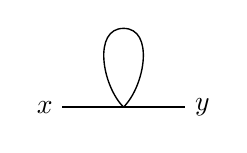
\begin{tikzpicture}
				\begin{feynhand}
					\vertex  (a) at(-1, 0) {$x$};
					\vertex  (b) at (1, 0) {$y$};
					\vertex (c) at (0, 0);
					\vertex (d) at (0, 1);
					\propag [plain] (a) to (b);
					\propag [plain] (c) to [out=45, in=0] (d) to [out=180, in=135] (c);
				\end{feynhand}
			\end{tikzpicture}
			=
			-\i\lambda\int \dd[4]{z} D(x-z)D(z-y)D(z_1-z_2) -\i\lambda\int \dd[4]{z} D(x-z)D(z-y)D(z_2-z_1)
		\end{equation}
		わかりやすさのために,まず区別して$z_1$と$z_2$としたが,これらは同じもので,重み$1$で足さなければいけないので,Symmetry factor $2$で割る必要がある.
	\item 他にも,統計力学っぽいところがあって,例えば,\textref{4.52}の和と積を入れ替える一連の計算は分配関数を計算するときによく使うテクニックである.
	\item \textref{4.55}の一つ前の式の右辺
		\begin{equation}
			\mel{\Omega}{\T(\phi(x)\phi(y))}{\Omega}\lim_{T\to\infty(1-\i\varepsilon)}(\abs{\braket{0}{\Omega}}^2e^{-\i E_0 2T})
		\end{equation}
		について,$\mel{\Omega}{\T(\phi(x)\phi(y))}{\Omega} $は外点につながっているdiagramの和で,$\e^{-\i E_0 2T}$は真空泡と議論があるが,忘れ去られている
		$\abs{\braket{0}{\Omega}}^2$は\textref{4.55}の比例に吸収させると思う.
	\item \textref{4.58}は今まで浸かっていた``disconnected''というワードは外点にdisconnectedの意味で使われていたが,
		このように二つに別れてしまうdiagramのこともdisconnectedというので,注意が必要であることをいう.
		前者は以前の議論で,分母分子でキャンセルするのでcorrelation functionに寄与しないのに対し,後者は
		correlation functionに寄与するという違いがある.
	\item \textref{4.64}は,不安定状態を考えているので,$p^0\neq E_{\vec{p}}=\sqrt{\vec{p}^2 + m^2}$であることに注意して,
		\begin{align}
			\frac{1}{p^2-m^2 + \i m\Gamma}
			& = \frac{1}{(p^0)^2 - E_{\vec{p}}^2  +\i m\Gamma}\\
			& \sim \frac{1}{2E_{\vec{p}}(p^0-E_{\vec{p}}) + \i m\Gamma}\label{eq:on-shell_approx}\\
			& = \frac{1}{2E_{\vec{p}}(p^0-E_{\vec{p}}+\i m\Gamma/(2E_{\vec{p}}))}
		\end{align}
		となる.Eq. \eqref{eq:on-shell_approx}では
		$p^0$が$E_{\vec{p}}$に近いとしている.
	\item Peskinのin, out stateは相互作用場で$T\to \pm\infty$にしたと定義されているが,
		他の本\cite{Kugo1989}, \cite{Sakamoto2020}では$T\to\pm \infty$で自由場と一致しているとして,定めているので,in, out場の定義が違うので,注意が必要である.あとで,相互作用場での$\ket{\vec{p}}$を自由場での$\ket{\vec{p}}_0$で表す操作をするが,そちらが通常のin, out場の定義である.
	\item \textref{4.68}のimpact parameterによるphaseのずれだが,通常の平行移動とおもうと,指数の方はプラスで出るように思う.
		しかし,$k_{\mathcal{B}}$の全空間で積分しているし,これは先の計算でデルタ関数として現れるだけなので,
		あまり議論に影響はしない.

	\item \textref{4.70}のS-matrixの定義は,二行目から見るのがわかりやすくて,同じ時間$t=0$で$\ket*{\vec{k}_{\mathcal{A}}\vec{k}_{\mathcal{B}}}$と$\bra{\vec{p}_1\vec{p}_2\cdots}$があって,
		$\ket*{\vec{k}_{\mathcal{A}}\vec{k}_{\mathcal{B}}}$を$H$で$-T$時間発展させたのがin stateで
		$\bra{\vec{p}_1\vec{p}_2\cdots}$を$T$時間発展させたのがout stateである.
	\item S-matrixを考えれば良いのだが,常に存在する自明な項があるので,この本ではそれを除いて考える.
		常に出てくる項とは
		\begin{enumerate}
			\item $\mathsf{S} = 1 + \i \mathsf{T}$
				\footnote{$\mathsf{S}$をscattering matrix, $\mathsf{T}$をtransfer matrixと言う.日本語ではそれぞれ散乱行列と転送行列であり,その$\mathsf{S}$と$\mathsf{T}$であるとゼミでボケようと思ったが,それまでに炎上したので自粛した.余裕のある人はこのネタを供養してください.}
				と分けたときの,$1$
			\item 運動量保存の$(2\pi)^4\delta^{(4)}(p_{\mathcal{A}}+p_{\mathcal{B}} - \sum_fp_f)$\footnote{out stateの添字に$f$を使っているのは,final stateのfだと思う.}
		\end{enumerate}
		である.これらを除いたものがinvariant matrix element $\M$である.
	\item \textref{4.74}は運動量状態$\prod_f 1/\sqrt{2E_f}\ket{\vec{p}_1\cdots}$へのamplitudeを求めている.
		なぜ,\textref{4.68}の$\phi_f(\vec{p}_f)$などがないのかと悩んだが,これは波束をFourier変換したときの
		展開係数なので単なる一つのモードを考えている今は当然必要ない.
		また,$1/\sqrt{2E_f}$はLorentz不変なnormalizationのためのfactorで,求めたいのは確率なので,二乗すると,必要な式を得る.
	\item \textref{4.76}の$\dd{\sigma}$を求める計算は,まず$\bar{k}_i$の6つの積分をまず計算することで,barのついている変数がデルタ関数で潰れることを確認する.
		
		まず,ここではimplicitにビーム方向に$z$軸をとって,impact parameter方向の二次元を$\perp$と取っている.ここで,$\bar{k}_{\mathcal{B}}^{\perp}$積分で$\bar{k}_{\mathcal{B}}^{\perp} = k_{\mathcal{B}}^{\perp}$を得て,
		これと,前のデルタ関数の結果を先取りすることで,$\bar{k}_{\mathcal{A}}^{\perp} = \sum_fp_f^{\perp} - k_{\mathcal{B}}^{\perp} = k_{\mathcal{A}}$となる.

		z成分は\textref{4.77}の計算が必要だが,ここで使っているデルタ関数の公式は
		\begin{equation}
			\delta(f(x)) = \sum_{\text{zeros}}\frac{1}{\abs{f'(x)}}\delta(x-x_0)
		\end{equation}
		と全ての零点を拾わなければならないが,ここでは和がない.
		デルタ関数のなかにある$\bar{k}_{\mathcal{A}}^z$についての関数の零点は,一般に2つあることが予期されるので正確にはこれではいけないはずである.

		これは次のように解釈できる.今の状況は運動量が狭い範囲にある波束を考えているので,
		その範囲は零点を一つしか拾わないように設定されていると思う.
		実際,次の計算でそのような近似を使うので,そこまでは和の状況で残しておき,そこでひとつだけ零点を拾うという議論のほうが筋は良い気がする.

		今の積分は$\delta(\bar{E}_{\mathcal{A}} + \bar{E}_{\mathcal{B}}-\sum_fE_f)$で$\bar{k}_{\mathcal{A}}^z = \sum_fp_f^z - \bar{k}_{\mathcal{B}}^z$となっているものを計算していて,
		\begin{align}
			&\sqrt{(k_{\mathcal{A}}^{\perp})^2+(\textcolor{red}{\bar{k}_{\mathcal{A}}^z})^2+m_{\mathcal{A}}^2} + \sqrt{(k_{\mathcal{B}}^{\perp})^2 + (\sum_fp_f^z-\textcolor{red}{\bar{k}_{\mathcal{A}}^z})^2+m_{\mathcal{B}}^2}\\
			& = \sum_fE_f = E_{\mathcal{A}} + E_{\mathcal{B}}\\
			& = \sqrt{(k_{\mathcal{A}}^{\perp})^2+(\textcolor{red}{k_{\mathcal{A}}^z})^2+m_{\mathcal{A}}^2} + \sqrt{(k_{\mathcal{B}}^{\perp})^2 + (\sum_fp_f^z-\textcolor{red}{k_{\mathcal{A}}^z})^2+m_{\mathcal{B}}^2}
		\end{align}
		であるので,$\bar{k}_{\mathcal{A}}^z = k_{\mathcal{A}^z}$となり,
		$\bar{k}_{\mathcal{B}}^z = \sum_fp_f^z-k_{\mathcal{A}}^z = k_{\mathcal{B}}^z$となる.
		これで,$\vec{\bar{k}}_{i}^z = \vec{k}_i^z$が言えるので,エネルギーについても$\bar{E}_i=E_i$となり,
		\textref{4.78}のように二乗でまとめることができる.
	\item $k/E = v$の書き換えは,静止系からLorentz変換したことを考えると
		\begin{equation}
			\mqty(\gamma & \gamma\beta\\ \gamma\beta & \gamma)\mqty(m\\0) = \mqty(E\\k)
		\end{equation}
		なので,$k/E = \beta = v$となる.

	\item \textref{4.82}でもデルタ関数の公式を使って,$\delta(E_{\text{CM}}-E_1-E_2)=(p_1/E_1 + p_1/E_2)^{-1}\delta(p-p_0)$としているが,これも真面目に考えるとおかしくて,$p_1$積分は$0\to \infty$で零点を計算をするとプラスマイナスの組ででてくるので複数拾うことはないにしろ,$E_{\text{CM}} < m_1+m_2$だと解を持たないのでゼロになる.
		零点をしらべるより,デルタ関数を変数変換して調べたほうがわかりやすくて\cite{Schwartz:2014sze},$x\coloneqq \sqrt{p_1^2+m_1^2} + \sqrt{p_1^2 + m_2^2} - E_{\text{CM}}$すると,
		\begin{equation}
		\int_{m_1+m_2-E_{\text{CM}}}^{\infty}\delta(x)
		\end{equation}
		となるが,これは$m_1+m_2 > E_{\text{CM}}$だと$0$を拾わない.
		
		しかし,これは物理的に考えるとtotal energyがmassより小さかったら,そのような散乱は起こらず興味のない結果になってしまうので,これが満たされているのは当然とも思える.
	\item \textref{4.102}の$1/2$のfactorはloopのsymmetry factorで割っている.

	\item Fermionの一粒子状態を$\ket{\vec{p}, s}$と書いただけでは$(a_{\vec{p}}^s)^{\dagger}\ket{0}$のfermionか$(b_{\vec{p}}^s)\ket{0}$のantifermionか区別がつかない.
		これで良いのかと聞いたところ,そもそも実用的にはまずdiagramを直接書いて計算するので,この記法を使った縮約の式に戻ることは殆ど無いそうである\footnote{ただし,symmetry factorを調べるときはdiagramだけだと探し漏れがあるので,
		その場合は縮約の式に戻って調べるという使い方をするそう.}.ここは,教育的配慮と認識して,上手く解釈するのが吉.
	\item \textref{4.115}で
		\begin{equation}
			\wick{\langle \c5{\vec{p}'}, \c2{\vec{k}'}\rvert \c2{\bar{\psi}_x}\c3{\psi_x}\c1{\phi_x}\c5{\bar{\psi}_y}\c4{\psi_y}\c1{\phi_y}\lvert \c4{\vec{p}}, \c3{\vec{k}}\rangle} 
		\end{equation}
		の縮約で,$\bar{\psi}$が入れ替わっている箇所があるように思うが,p. 119で説明があるように$\bra*{\vec{p}', \vec{k}'} = \bra{0}a_{\vec{k}'}a_{\vec{p}'}$と外れるので,この計算はあっている.
		また,spinorの順番が$\bar{u}u\bar{u}u$になっているのは当然で,$u$は4成分あるので,この順番でないと1成分に縮約できない.
	\item \textref{4.130}の$\partial^2A_{\mu} = 0$のゲージのとり方をLorentz gaugeと書いてあるが,Lorenzである
		\footnote{日本語だと前者をローレンツ,後者をローレンスと表記することが多いと思う.}.
	\item Chapter 4.8の力の働き方が引力か斥力かという話は,\cite{Zee:2003mt}の一章にも経路積分形式で書かれている.
	\item \textref{4.132}は
		\begin{equation}
			\intp[4]{q}\frac{\i g_{\mu\nu}}{q^2+\i\epsilon}\e^{-\i q(x-y)}
			= \intp{q}(\i g_{\mu\nu})\e^{\i\vec{q}\cdot (\vec{x}-\vec{y})}\int\frac{\dd{q^0}}{2\pi} \frac{\e^{- \i q^0(x^0-y^0)}}{(q^0)^2-\abs{\vec{q}}^2 + \i\epsilon}
		\end{equation}
		として,後ろの計算を留数積分でする.

		\begin{equation}
			I  =\int \dd{z}\frac{\e^{-\i zx}}{z^2-z_0^2 + \i\epsilon}
		\end{equation}
		は$z = \pm\sqrt{z_0^2-\i\epsilon}$にsimple poleがあり,下半平面で積分路を閉じると収束するので,$z = \sqrt{z_0^2-\i\epsilon}\sim \abs{z_0}$の方のpoleを拾って,
		\begin{equation}
			I = -2\pi\i\frac{\e^{-\i zx}}{2z}
		\end{equation}
		なので教科書の結果を得る.
	\item \textref{4.133}の計算を縮約に戻ってやると次のようになる.
		\begin{align}
			&\i \M (2\pi)^4\delta^{(4)}(p+k -p'-k')
			\\&= 
			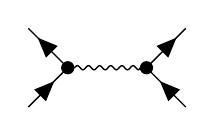
\begin{tikzpicture}[baseline=(x.base)]
				\begin{feynhand}
					\vertex [dot] (x) at (-0.5, 0) {};
					\vertex [dot] (y) at (0.5, 0) {};
					\vertex (p) at (-1, -0.5);
					\vertex (p') at (-1, 0.5);
					\vertex (k) at (1, -0.5);
					\vertex (k') at (1, 0.5);
					\propag[fermion] (p) to (x);
					\propag[fermion] (x) to (p');
					\propag[fermion] (k) to (y);
					\propag[fermion] (y) to (k');
					\propag[photon] (x) to (y);
				\end{feynhand}
			\end{tikzpicture}\\
			&= \bra{0}\wick{\c2{a_{k'}}\c4{a_{p'}}\qty(-\i e\int \dd[4]{x})\c4{\bar{\psi_x}}\gamma^{\mu}\c3{\psi_x}\c5{A_\mu}\qty(-\i e\int\dd[4]y)\c2{\bar{\psi_y}}\gamma^{\nu}\c1{\psi_y}\c5{A_\nu}\c3{a_p^{\dagger}}\c1{a_k^{\dagger}}}\ket{0}\\
			&= (-\i e)^2\int \dd[4]{x}\int \dd[4]{y}\bra{0}\wick{\c2{a_{k'}}\c4{a_{p'}}\c4{\bar{\psi_x}}(-1)\c2{\bar{\psi_y}}\gamma^{\mu}\c5{A_\mu}\gamma^{\nu}\c1{\psi_y}\c5{A_\nu}(-1)\c3{\psi_x}\c3{a_p^{\dagger}}\c1{a_k^{\dagger}}}\ket{0}\\
			&= (-\i e)^2\int\dd[4]{x}\int \dd[4]{y}\intp[4]{q}
			\bar{u}(p')\e^{\i p'x}\gamma^{\mu}u(p)\e^{-\i px}\frac{-\i g_{\mu\nu}}{q^2+\i\epsilon}\e^{-\i q(x-y)}\bar{u}(k')\e^{\i k'y}\gamma^{\nu}u(k)\e^{-\i kx}\\
			&= (-\i e)^2\intp[4]{q}\bar{u}(p')\gamma^{\mu}u(p)\frac{-\i g_{\mu\nu}}{q^2+\i\epsilon}\bar{u}(k')\gamma^{\nu}u(k)(2\pi)^4\delta^{(4)}(p+q-p')(2\pi)^4\delta^{(4)}(k-q-k')\\
			&= (-\i e)^2\bar{u}(p')\gamma^{\mu}u(p)\frac{-\i g_{\mu\nu}}{(p'-p)^2}\bar{u}(k')\gamma^{\nu}u(k) (2\pi)^4\delta^{(4)}(p+k-p'-k')
		\end{align}
		となり,常に出てくる外線の運動量保存を省いたものが\textref{4.133}である\footnote{もっと丁寧にやるべきところは,gamma行列とspinorのspinor添字をちゃんと書いて,行列の積の順序がこれで良いか確かめることである.}.

\end{itemize}

	\section{Elementary Process of Quantum Electrodynamics}
\begin{itemize}
	\item $\i\M = (\i\e^2/q^2)\bar{v}(p')\gamma^{\mu}u(p)\bar{u}(k)\gamma_{\mu}v(k')$だが,cross sectionを求める際は$\abs{\M}^2$が必要で,$(\bar{v}\gamma^{\mu}u)^{*}$が必要であるが,これはbarのnotationが優れているポイントで,
		$(\gamma^0)^{\top} = \gamma^{0}$, $(\gamma^{i})^{\top} =- \gamma^{i}$であるので,$(\bar{v}\gamma^{\mu}u)^{*} = \bar{u}\gamma^{\mu}v$である.
	\item p.132でspinの向きを指定せず平均をとる操作をするが,これは始状態の$\mathrm{e^+}$, $\mathrm{e^-}$に対してであり,終状態の$\mathrm{\mu^+}$, $\mathrm{\mu^-}$については和をとるので,$1/2$のfactorは$s$, $s'$についての和に関してかかり,\textref{5.4}では全体で$1/4$のfactorがかかる.
	\item \textref{5.4}での$\tr$はスピノル添字に関してのtraceであることに注意.$\mu$などはベクトルの添字なのでtraceには関係しない.
	\item $\tr\qty((\slashed{p} -m_{\elec})\gamma^{\mu}(\slashed{p}+m_{\elec}\gamma^{\nu})) = 4\qty((p')^\mu p^\nu + (p')^\nu p^\mu - g^{\mu\nu}(p\cdot p' + m_\elec^2))$
		は$\slashed{p} = \gamma^{\mu} p_\mu$に注意して,Gamma行列に対してのTraceの公式を使えば導ける.
	\item \textref{5.6}の等式はあとで使う.一番最後の$\epsilon^{\alpha\beta\mu\nu} \epsilon_{\alpha\beta\rho\sigma} = -2(\delta\indices{^\mu_\rho}\delta\indices{^\nu_\sigma} - \delta\indices{^\mu_\sigma}\delta\indices{^\nu_\rho})$から示す.

		まず,これはすでに$\alpha$, $\beta$に関して和を取られているので,$\mu$, $\nu$が$\alpha$, $\beta$と一致すると完全反対称性からゼロになる.つまり,$\mu$ ($\nu$)は$\rho$か$\sigma$と一致しなければならない.また,$\mu$と$\nu$, $\rho$と$\sigma$は反対称なので,反対称に組まなければいけない.
		これらから$\epsilon^{\alpha\beta\mu\nu} \epsilon_{\alpha\beta\rho\sigma} \propto \delta\indices{^\mu_\rho}\delta\indices{^\nu_\sigma} - \delta\indices{^\mu_\sigma}\delta\indices{^\nu_\rho}$である.
		
		比例定数$c$は$\mu$, $\nu$, $\rho$, $\sigma$に適当な文字を入れて決定すればよい.$(\mu, \nu) = (\rho, \sigma) = (2, 3)$として,
		$\epsilon^{0123}\epsilon_{0123}  + \epsilon^{1023}\epsilon_{1023} = -2$\footnote{$\epsilon^{0123} = 1$とする規約で,
		全ての添字を下ろすと,
		空間成分$1$, $2$, $3$を下ろすときに奇数回$-1$が出るので,
		$\epsilon_{0123} = -1$}.
		一方,$c(\delta\indices{^2_2}\delta{^3_3} - \delta{^2_3}\delta{^3_2}) = a$より$c = -2$であるので,主張は示された.
	\item \textref{5.7}の等式は$\gamma^{\mu}$の数$n$が偶数のとき成り立つ.
		奇数ならば,\textref{5.5}の二番目の式からゼロになる.
		$\gamma^5$が入った場合もなりたつと書いてあるが,$\gamma^{5}$の個数は$n$にカウントしないと思う.また,$\gamma^5$が入ったとき$n$が奇でもゼロになるとは言えない.例えば$n=4$のとき$\epsilon^{\mu\nu\rho\sigma}$に比例する.
\end{itemize}

	\section{Radiative Corrections: Introduction}
\begin{itemize}
    \item このセクションは,書いてあるとおりに計算すればたくさん発散が出てきて死ぬセクションらしい.
\end{itemize}
\subsection{Soft Bremsstrahlung}

	\bibliography{QFT}
	\bibliographystyle{ytamsalpha}
	%\bibliographystyle{ytamsbeta}
\end{document}
